\chapter{METODOLOGI}

% Ubah konten-konten berikut sesuai dengan isi dari metodologi

\section{Metode yang digunakan}

Dalam penyelesaian tugas akhir ini, diperlukan penggunaan suatu metode tertentu yang akan menjadi dasar selama proses pengerjaan. Untuk memperkuat penggunaan metode tersebut, diperlukan serangkaian langkah yang tergambar dalam diagram alir sebagai berikut.

% % Contoh input gambar dengan format *.jpg
\begin{figure} [H] \centering
  % Nama dari file gambar yang diinputkan
  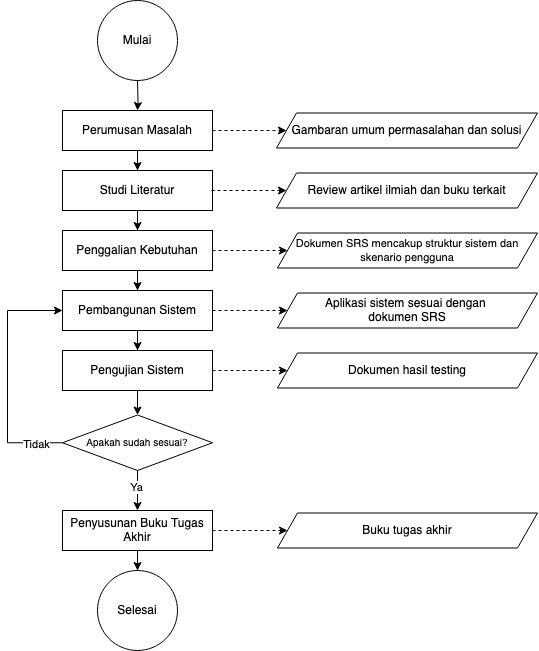
\includegraphics[scale=0.5]{gambar/flow.png}
  % Keterangan gambar yang diinputkan
  \caption{Diagram alir tugas akhir}
  % Label referensi dari gambar yang diinputkan
  \label{fig:Flow}
\end{figure}

\subsection{Perumusan Masalah}
Langkah pertama dalam tugas akhir ini adalah mengidentifikasi perumusan masalah. Proses penentuan perumusan masalah didasarkan pada latar belakang permasalahan yang sedang dihadapi. Hasil akhir dari proses ini adalah perumusan masalah untuk menciptakan suatu sistem integrasi data dengan menggunakan metode ETL.

\subsection{Studi Literatur}
Saat melakukan studi literatur, peneliti melakukan pencarian dalam berbagai bentuk sumber seperti jurnal, buku, dan referensi lainnya untuk memberikan dukungan dalam menyelesaikan tugas akhir ini. Rentang waktu sumber referensi ini dibatasi hingga maksimal sepuluh tahun dari tahun penulisan penelitian ini. Beberapa referensi yang penting bagi penulis dalam tugas akhir ini meliputi topik integrasi data, heterogenitas data, metode ETL, serta konsep pemrograman aplikasi seperti EletronJS, Python, dan SQLite Database.

\subsection{Penggalian Kebutuhan}
Tahap penggalian kebutuhan melibatkan pengumpulan data tentang kebutuhan sistem integrasi data dari pengguna akhir. Jenis kebutuhan ini terbagi menjadi fungsional dan nonfungsional. Kebutuhan fungsional menjadi inti dari pengembangan sistem integrasi data, sementara kebutuhan nonfungsional mendukung implementasinya. Hasil dari penggalian ini akan disusun menjadi dokumen Software Requirement Specification (SRS) yang mencakup struktur sistem dan skenario pengguna dari sistem yang sedang dikembangkan. Skenario pengguna yang dihasilkan dapat ditemukan dalam Gambar \ref{fig:Use-case}, sedangkan rancangan struktur sistem yang diperlukan untuk penelitian ini terdapat dalam Gambar \ref{fig:structure-system}.


\begin{figure} [H] \centering
  % Nama dari file gambar yang diinputkan
  
\includegraphics[scale=0.4]{gambar/ph.jpg}
  % Keterangan gambar yang diinputkan
  \caption{Diagram Use-case aplikasi}
  % Label referensi dari gambar yang diinputkan
  \label{fig:Use-case}
\end{figure}

\begin{figure} [H] \centering
  % Nama dari file gambar yang diinputkan
  
\includegraphics[scale=0.4]{gambar/ph.jpg}
  % Keterangan gambar yang diinputkan
  \caption{Diagram struktur sistem}
  % Label referensi dari gambar yang diinputkan
  \label{fig:structure-system}
\end{figure}


\subsection{Pembangunan Sistem}
Tahapan Pembangunan sistem dilakukan secara bertahap, mengikuti urutan atau prioritas yang telah ditetapkan pada tahap penggalian kebutuhan. Selama pembangunan sistem, perhatian khusus diberikan pada keseluruhan use-case yang telah disusun sebelumnya. Pembangunan sistem ini terstruktur dalam enam komponen utama dengan rincian sebagai berikut:
\begin{enumerate}
  \item \subsubsection*{Penanganan Sumber Data}
  Komponen ini memungkinkan pengguna untuk memasukkan data sumber SQL seperti Mysql atau PostgreSQL dan menyimpannya sebagai "Source" dalam sistem seperti pada proses di Gambar. Pada komponen ini akan disediakan antarmuka di mana pengguna dapat memasukkan detail data sumber seperti string koneksi, kredential yang meliputi username dan password. Sistem akan melakukan verifikasi pada data masukan untuk memastikan bahwa format data sesuai dengan jenis sumber data yang dimasukkan, sebagai contoh user wajib menuliskan user dan password apabila pengguna ingin memasukkan basis data Mysql sebagai "Source" tersebut. Setelah itu sistem menyimpan hasil masukkan pengguna ke dalam basis data lokal yang tergabung pada sistem.
  \item \subsubsection*{Pembuatan Koneksi Migrasi}
  Komponen ini Memungkinkan pengguna untuk membuat koneksi migrasi antara sumber dan tujuan yang telah ditentukan dalam sistem seperti pada Gambar. Basis data tujuan atau "Destination" merupakan basis data central yang menjadi tujuan integrasi data ini. Pada proses pembuatan koneksi, pengguna diharuskan memilih tabel yang akan dimigrasi dari basis data sumber ke basis data tujuan. Sistem akan melakukan ekstrasi metadata pada tabel yang dipilih guna mendapatkan informasi kolom tabel.
  \item \subsubsection*{Modul Ekstraksi Metadata Tabel}
  Komponen ini mengekstraksi informasi metadata untuk tabel-tabel yang dipilih dari database sumber. Proses pengambilan metadata memanfaatkan API database sesuai dengan sistem basis data yang dipilih.
  \item \subsubsection*{Modul Migrasi Data}
  Komponen ini merupakan bagian utama dari aplikasi, yaitu proses ETL yang melibatkan proses perpindahan data dari sumber ke database tujuan. Tahapan migrasi mencakup tiga aktivitas, yaitu,
    \begin{enumerate}
      \item ekstraksi data,
      \item transformasi data,
      \item muat data
    \end{enumerate}
  
  \item \subsubsection*{Modul Monitoring dan Manajemen Koneksi Migrasi}
  Komponen ini bertanggung jawab untuk memantau jalannya proses migrasi, mendeteksi dan menangani masalah yang mungkin timbul, serta memberikan laporan dan statistik terkait kinerja sistem. Pada komponen ini, sistem memantau status koneksi dan memberikan umpan balik kepada pengguna. Selain itu, komponen ini menyediakan fitur yang memungkinkan pengguna untuk memulai kembali koneksi jika terputus.
\end{enumerate}


\subsection{Pengujian Sistem}
Tahap pengujian sistem merupakan langkah penting yang dilakukan oleh penulis untuk memeriksa fungsi dari sistem integrasi yang sedang dikembangkan. Tahap pengujian ini sebaiknya dilakukan bersamaan dengan proses pengembangan guna memastikan bahwa sistem informasi beroperasi sesuai yang diharapkan. Pengujian sistem dilakukan dua kali. Pertama, pengujian unit (unit testing) digunakan untuk mengevaluasi kehandalan sistem yang telah dibuat berdasarkan skenario use-case yang telah ditetapkan sebelumnya. Tujuan dari pengujian ini adalah memastikan bahwa setiap fitur berjalan dengan baik dan sesuai fungsinya dalam sistem. Selain itu, pengujian ini juga memverifikasi kinerja fitur-fitur tersebut dengan melakukan pengawasan pada proses internal sistem. Kedua, pengujian penerimaan (acceptance testing) dilakukan untuk mengamati tanggapan pengguna akhir ketika menggunakan versi beta dari sistem yang telah dibuat. Pengujian ini bertujuan untuk memahami reaksi dan pengalaman pengguna dalam menggunakan sistem yang dikembangkan. Metode black-box testing digunakan pada pengujian ini, di mana pengguna akhir tidak perlu memiliki pengetahuan tentang detail teknis kode yang digunakan oleh sistem. Dalam keseluruhan proses pengujian ini, fokus utama adalah memastikan bahwa sistem tidak hanya berfungsi dengan baik dari perspektif teknis, tetapi juga memenuhi kebutuhan dan ekspektasi pengguna akhir.

\subsection{Penyusunan Buku Tugas Akhir}
Tahap akhir dari penyelesaian tugas akhir ini adalah penyusunan buku tugas akhir yang berfungsi sebagai laporan formal dari peneliti kepada perguruan tinggi, mendokumentasikan penelitian yang telah dilakukan dalam periode tertentu. Selain buku tugas akhir, ada kemungkinan untuk membuat beberapa dokumen tambahan yang juga berperan dalam mendokumentasikan keseluruhan penelitian ini.


% Contoh penggunaan referensi dari gambar yang diinputkan
% Pada \emph{blueprint} yang tertera di Gambar \ref{fig:Blueprint}. \lipsum[12]

\section{Urutan pelaksanaan penelitian}
% Ubah tabel berikut sesuai dengan isi dari rencana kerja
\newcommand{\w}{}
\newcommand{\G}{\cellcolor{gray}}
\begin{table}[H]
  \captionof{table}{Tabel timeline}
  \label{tbl:timeline}
  \begin{tabular}{|p{2.5cm}|c|c|c|c|c|c|c|c|c|c|c|c|c|c|c|c|c|c|c|c|}

    \hline
    \multirow{3}{*}{Kegiatan} & \multicolumn{20}{|c|}{Bulan}                                                                 \\
    \cline{2-21}  & \multicolumn{4}{|c|}{I} & \multicolumn{4}{|c|}{II} & \multicolumn{4}{|c|}{III} & \multicolumn{4}{|c|}{IV} & \multicolumn{4}{|c|}{V} \\
    \cline{2-21}              &
    1                         & 2                             & 3  & 4  & 1  & 2  & 3  & 4  & 1  & 2 & 3 & 4 & 1  & 2 & 3 & 4 & 1  & 2 & 3 & 4 \\
    \hline

    % Gunakan \G untuk mengisi sel dan \w untuk mengosongkan sel
    Perumusan Masalah          &
    \G                        & \G                            & \G & \G & \w & \w & \w & \w & \w & \w & \w & \w & \w & \w & \w & \w & \w & \w & \w & \w \\
    \hline
  \end{tabular}
\end{table}

Pada \emph{timeline} yang tertera di Tabel \ref{tbl:timeline} \lipsum[10]
